\chapter{算符、可观测量与泡利矩阵}

好的记号不是装饰。在一门由抽象矢量与复数构建的学科中，一种能让我们移动符号而不必反复把它们翻译成文字的记号，本身就是机械装置的一部分。狄拉克的bra--ket记号之所以有价值，正是因为这个原因：它让态空间的几何保持可见，同时允许我们用分量和矩阵进行计算。

我们当前的任务是数学性的。我们将引入线性算符，学习它们如何作用于bra以及ket，并分离出称为厄米算符的特殊类别。只有到那时，我们才会附上物理词语\emph{可观测量}、\emph{测量结果}和\emph{概率}。回报是，三个自旋可观测量作为泡利矩阵出现，而不是作为需要记忆的对象交给我们。

\section{正交归一基与分量}

态构成一个复线性矢量空间。它的ket矢量可以相加，也可以乘以复数。与每个ket\(\ket{A}\)相伴的是一个bra\(\bra{A}\)，通过共轭对偶运算得到。基不是唯一的，但一旦选定了一个基，每个矢量都可以用它在该基中的分量来描述。

设
\[
\bigl\{\ket{1},\ket{2},\ldots,\ket{N}\bigr\}
\]
为一个正交归一基。正交性与归一性概括为
\begin{equation}
\braket{j}{i}=\delta_{ji}.
\label{eq:orthonormal-basis}
\end{equation}
这里，当\(j=i\)时\(\delta_{ji}\)为1，否则为0。维数\(N\)是空间中相互正交方向的最大数目；一个完备正交归一基恰好包含这么多个矢量。

将任意ket展开为
\begin{equation}
\ket{A}=\sum_i \alpha_i\ket{i}.
\label{eq:ket-expansion}
\end{equation}
这些系数并不神秘。从左边乘以\(\bra{j}\)：
\begin{align}
\braket{j}{A}
 &=\sum_i\alpha_i\braket{j}{i} \\
 &=\sum_i\alpha_i\delta_{ji}
 =\alpha_j.
\end{align}
因此
\begin{equation}
\alpha_i=\braket{i}{A}.
\label{eq:components-inner-products}
\end{equation}
第\(i\)个分量是\(\ket{A}\)在第\(i\)个基方向上的投影。

将式~\eqref{eq:components-inner-products}代回式~\eqref{eq:ket-expansion}，得到特别有用的形式
\begin{equation}
\ket{A}=\sum_i\ket{i}\braket{i}{A}.
\label{eq:ket-completeness-action}
\end{equation}
这个求和没有对矢量做任何事情；它只是把矢量分解到其基方向上，然后再把它重建起来。我们将反复使用这个操作。它通常被描述为\emph{插入一组完备态}，因为
\begin{equation}
\sum_i\ket{i}\bra{i}=\mathbf 1.
\label{eq:resolution-identity}
\end{equation}

相应的bra展开为
\begin{equation}
\bra{A}=\sum_i\braket{A}{i}\bra{i}
       =\sum_i\alpha_i^*\bra{i}.
\label{eq:bra-expansion}
\end{equation}
\(\alpha_i\)上的复共轭是必不可少的。把一个ket反转为bra会对每个数值系数取共轭。

\begin{figure}[htbp]
\centering
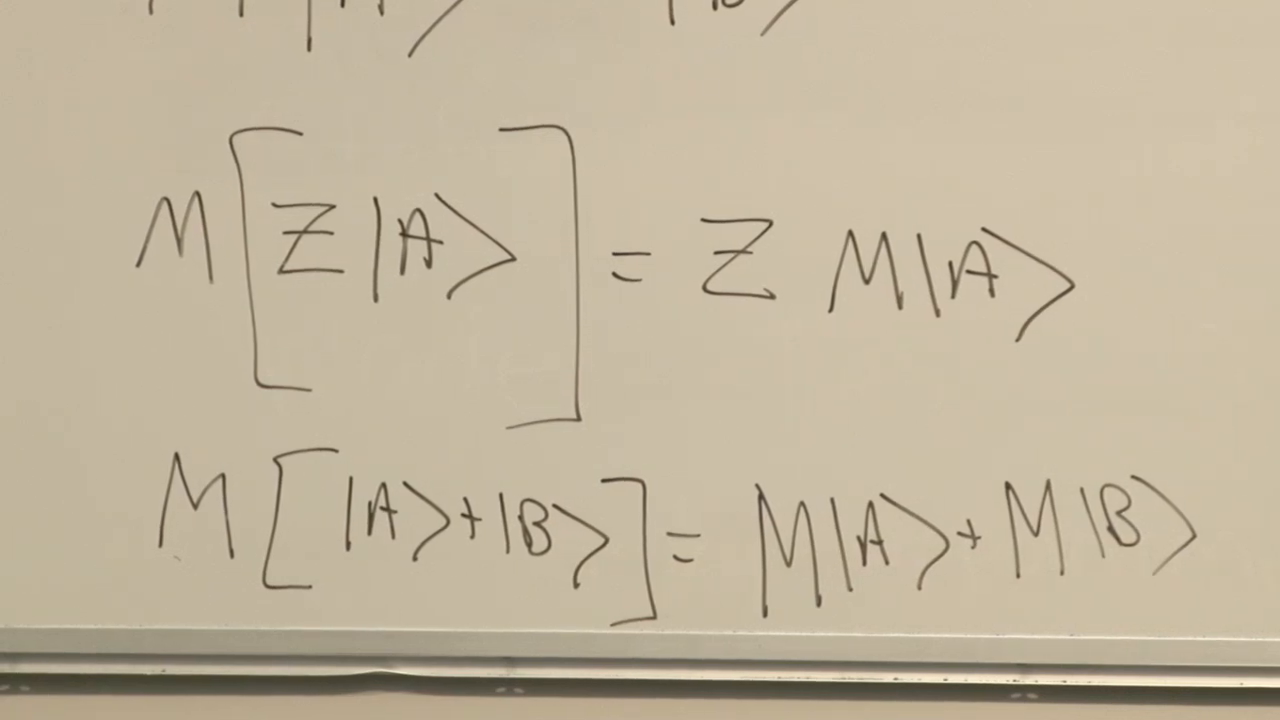
\includegraphics[width=0.82\textwidth]{lecture_03_figure_04.png}
\caption{线性算符的两条定义规则，写在基的回顾之后。}
\lectureframe{00:12:44}
\end{figure}

\section{作为机器的线性算符}

线性算符\(M\)是一条规则，它把一个输入ket变成一个唯一的输出ket。约翰·惠勒给出的一个有用图像是一台带有输入端口和输出端口的机器：插入\(\ket{A}\)，转动轮子，得到\(M\ket{A}\)。输出由输入决定。反过来不必唯一；两个输入可能产生同一个输出，而且逆机器不一定存在。

\emph{线性}这个形容词由两条规则组成。对于复数\(z\)，
\begin{align}
M\bigl(z\ket{A}\bigr)&=z\,M\ket{A}, \label{eq:operator-homogeneous}\\
M\bigl(\ket{A}+\ket{B}\bigr)&=M\ket{A}+M\ket{B}.
\label{eq:operator-additive}
\end{align}
标量原样通过机器，而和可以逐项处理。这些规则也意味着对任意有限复线性组合的线性性。

同样的想法适用于普通三维矢量。量子力学并没有发明线性映射。它使线性映射变得不可或缺，因为态空间是抽象且复的，并且因为可测量量将由一类特殊的这种映射来表示。

\section{从算符到其矩阵}

假设机器把\(\ket{A}\)送到\(\ket{B}\)：
\begin{equation}
M\ket{A}=\ket{B}.
\label{eq:operator-action}
\end{equation}
为输入和输出选择同一个正交归一基，并写出
\[
\ket{A}=\sum_j\alpha_j\ket{j},
\qquad
\ket{B}=\sum_i\beta_i\ket{i}.
\]
为了求出第\(i\)个输出分量，用\(\bra{i}\)对式~\eqref{eq:operator-action}作投影：
\begin{equation}
\bra{i}M\ket{A}=\braket{i}{B}=\beta_i.
\end{equation}
现在插入\(\ket{A}\)的展开：
\begin{align}
\bra{i}M\ket{A}
 &=\sum_j\bra{i}M\ket{j}\braket{j}{A}\\
 &=\sum_j\bra{i}M\ket{j}\alpha_j
 =\beta_i.
\end{align}
这些数
\begin{equation}
m_{ij}\equiv\bra{i}M\ket{j}
\label{eq:matrix-elements}
\end{equation}
是\(M\)在所选基中的\emph{矩阵元}。因此，
\begin{equation}
\boxed{\sum_jm_{ij}\alpha_j=\beta_i.}
\label{eq:component-action}
\end{equation}

\begin{figure}[htbp]
\centering
\includegraphics[width=0.84\textwidth]{lecture_03_figure_02.png}
\caption{抽象方程\(M\ket{A}=\ket{B}\)，经过投影并分解为分量规则\(\sum_jm_{ij}\alpha_j=\beta_i\)。}
\lectureframe{00:18:30}
\end{figure}

如果空间维数为\(N\)，那么\(N^2\)个数\(m_{ij}\)构成一个\(N\times N\)方阵。式~\eqref{eq:component-action}正是
\begin{equation}
\begin{pmatrix}
m_{11}&m_{12}&\cdots&m_{1N}\\
m_{21}&m_{22}&\cdots&m_{2N}\\
\vdots&\vdots&\ddots&\vdots\\
m_{N1}&m_{N2}&\cdots&m_{NN}
\end{pmatrix}
\begin{pmatrix}
\alpha_1\\
\alpha_2\\
\vdots\\
\alpha_N
\end{pmatrix}
=
\begin{pmatrix}
\beta_1\\
\beta_2\\
\vdots\\
\beta_N
\end{pmatrix}.
\label{eq:matrix-vector-action}
\end{equation}
为了得到\(\beta_1\)，将第一行乘以输入列并相加；对\(\beta_2\)用第二行重复，依此类推。矩阵是惠勒机器的具体版本。

\begin{figure}[htbp]
\centering
\includegraphics[width=0.84\textwidth]{lecture_03_figure_03.png}
\caption{同一个算符作用显示为方阵乘以输入系数列。}
\lectureframe{00:20:01}
\end{figure}

我们获得了一种算法，却失去了一些可见的几何。抽象陈述\(M\ket{A}=\ket{B}\)不依赖于坐标。具体的矩阵元\(m_{ij}\)、\(\alpha_j\)和\(\beta_i\)则确实依赖于所选基。不同的正交归一基会改变这三个数组，而底层的映射及其物理预言保持不变。

\begin{classroomqa}
\audiencequestion{基的选择能决定一个问题是否可解吗？}
\lecturerresponse{它能决定解是否容易看出。选得好的基可能使一个算符对角化，计算几乎立刻完成；选得差的基可能把结构隐藏在令人不快的代数运算之下。它不能改变实验结果。如果两个基给出不同的物理答案，那么计算就是错的。}
\end{classroomqa}

\section{左矢、右矢与反线性}

\begin{classroomqa}
\audiencequestion{线性算符能把一个右矢变成左矢，或把一个左矢变成右矢吗？}
\lecturerresponse{不能，刚刚定义的那种普通线性算符做不到。它把右矢映射为右矢，复标量原样穿过。交换右矢与左矢的运算还会对它们的系数取复共轭，因此它属于另一类。}
\end{classroomqa}

乘以一个固定复数是简单的线性算符。复共轭则不是。若用\(K\)表示共轭，则
\[
K\bigl(z\ket{A}\bigr)=z^*K\ket{A},
\]
而不是\(zK\ket{A}\)。这样的映射称为\emph{反线性}。这个名字并不意味着与线性相反；它记录的是对标量取共轭。它与反粒子之间更深层的联系超出了目前的讨论范围。

不过，线性算符也可以作用于左矢。按约定，算符写在右边：
\begin{equation}
\bra{A}M.
\end{equation}
这样定义是为了让矩阵元没有括号歧义：
\begin{equation}
\bra{A}\bigl(M\ket{B}\bigr)
=
\bigl(\bra{A}M\bigr)\ket{B}
\equiv
\bra{A}M\ket{B}.
\label{eq:bracket-independence}
\end{equation}

要看出为什么可以这样做，把两个矢量都展开：
\begin{align}
\bra{A}M\ket{B}
 &=\left(\sum_i\alpha_i^*\bra{i}\right)
   M
   \left(\sum_j\beta_j\ket{j}\right)\\
 &=\sum_{ij}\alpha_i^*m_{ij}\beta_j.
\label{eq:matrix-element-double-sum}
\end{align}
这是一个普通的二重和。我们可以先对\(j\)求和，把\(M\)看作作用于右矢；也可以先对\(i\)求和，把它看作作用于左矢。结果相同。记号正是这样安排的，以便去掉不必要的括号。

\section{匕首运算}

还有第二个不同的左矢侧问题。假设
\[
M\ket{A}=\ket{B}.
\]
什么算符把相应的左矢\(\bra{A}\)变成\(\bra{B}\)？一般不是\(M\)本身。如果\(M\)是乘以复数\(z\)，那么右矢方程会是\(\ket{B}=z\ket{A}\)，而左矢方程会是\(\bra{B}=z^*\bra{A}\)。

所需的算符记作\(M^\dagger\)，即\(M\)的\emph{厄米共轭}，定义为
\begin{equation}
M\ket{A}=\ket{B}
\quad\Longleftrightarrow\quad
\bra{A}M^\dagger=\bra{B}.
\label{eq:dagger-definition}
\end{equation}
匕首是复共轭在算符上的类比。

它的矩阵规则直接可得。令
\[
M\ket{i}=\ket{i'}.
\]
则
\[
m_{ji}=\bra{j}M\ket{i}=\braket{j}{i'}.
\]
取匕首后的左矢关系是\(\bra{i}M^\dagger=\bra{i'}\)，所以
\[
(m^\dagger)_{ij}
=\bra{i}M^\dagger\ket{j}
=\braket{i'}{j}.
\]
颠倒内积的顺序会对其取复共轭：
\[
\braket{i'}{j}=\braket{j}{i'}^*.
\]
因此
\begin{equation}
\boxed{(m^\dagger)_{ij}=m_{ji}^*.}
\label{eq:dagger-matrix-elements}
\end{equation}

\begin{figure}[htbp]
\centering
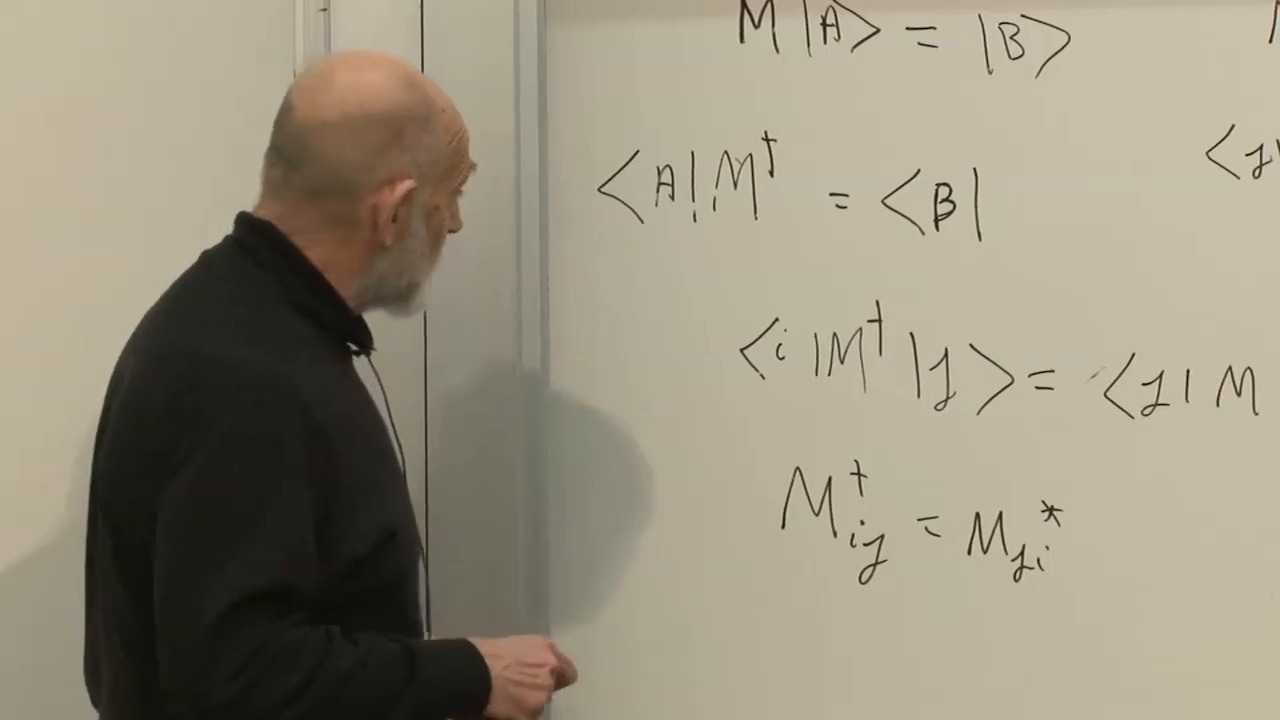
\includegraphics[width=0.84\textwidth]{lecture_03_figure_05.png}
\caption{厄米共轭的完整板书关系：交换指标并取复共轭。}
\lectureframe{00:42:23}
\end{figure}

用矩阵语言说，我们先转置再取复共轭：
\begin{equation}
\begin{pmatrix}
a&b\\
c&d
\end{pmatrix}^{\!\dagger}
=
\begin{pmatrix}
a^*&c^*\\
b^*&d^*
\end{pmatrix}.
\label{eq:dagger-two-by-two}
\end{equation}
转置把各矩阵元关于主对角线反射；共轭把每个\(i\)换成\(-i\)。例如，
\begin{equation}
\begin{pmatrix}
2&6+7i\\
4-i&9+i
\end{pmatrix}^{\!\dagger}
=
\begin{pmatrix}
2&4+i\\
6-7i&9-i
\end{pmatrix}.
\label{eq:dagger-numerical-example}
\end{equation}
对角元留在原位但被取共轭，而两个非对角元交换位置并被取共轭。

\section{厄米算符}

一个复数等于自身的复共轭，当且仅当它是实数。算符上的类比立刻可得。

\begin{definition}
算符 \(M\) 是\emph{厄米的}，当
\begin{equation}
M=M^\dagger.
\label{eq:hermitian-definition}
\end{equation}
时。
等价地，在每个正交归一基中，
\begin{equation}
m_{ij}=m_{ji}^*.
\label{eq:hermitian-components}
\end{equation}
\end{definition}

在方程~\eqref{eq:hermitian-components}中令\(i=j\)。于是
\[
m_{ii}=m_{ii}^*,
\]
所以每个对角元都是实数。非对角元则以共轭反射对的形式出现。若一个矩阵元是\(4-i\)，其反射伙伴就是\(4+i\)；若一个是实数\(5\)，其伙伴也是。

\begin{figure}[htbp]
\centering
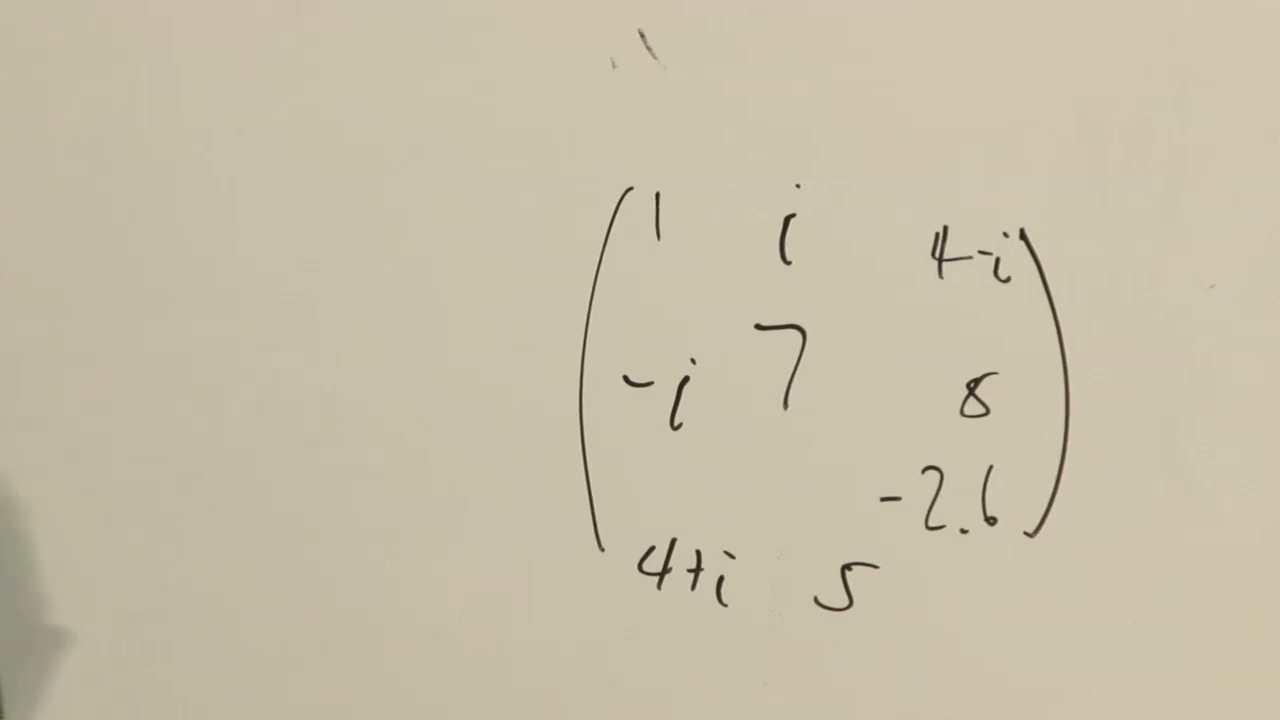
\includegraphics[width=0.78\textwidth]{lecture_03_figure_06.png}
\caption{一个完整的厄米矩阵示例：对角线上是实矩阵元，关于对角线反射的复共轭对。}
\lectureframe{00:45:43}
\end{figure}

厄米算符之所以重要，是因为它们将表示可测量。在作出这一认定之前，我们需要理解它们的本征方向。

\section{本征矢量与本征方向}

初次接触本征矢量时，这部分可能让人觉得比周围的物理内容进展得更快。这些观念是标准线性代数，而不是新的物理假设；如果不熟悉，值得安静地复习一下定义，然后再回到论证中来。

一般算符会改变矢量的方向。例如，普通三维空间中的旋转会使几乎每个矢量偏离自身。旋转轴是例外：沿该轴的矢量返回时方向不变。这就是本征矢量的模型。

实二维平面中的非平凡旋转展示了相反的可能性：没有任何实方向在实尺度范围内保持不变。因此，在受限实空间上的一般算符不必有实本征矢量。量子力学中使用的复状态空间上的厄米算符具有强得多的性质。

\(M\)的本征矢量满足
\begin{equation}
M\ket{i}=\lambda_i\ket{i}.
\label{eq:eigenvalue-equation}
\end{equation}
数\(\lambda_i\)是它的本征值。本征矢量属于算符；若不指明它保持方向的是哪个映射，就不能谈论本征矢量。

它的长度和相位不由式~\eqref{eq:eigenvalue-equation}固定。对每个非零复数\(z\)，
\[
M\bigl(z\ket{i}\bigr)
=zM\ket{i}
=\lambda_i\bigl(z\ket{i}\bigr).
\]
因此更准确的说法是\emph{本征方向}：\(\ket{i}\)的每个非零倍数描述同一方向并带有同一本征值。我们通常选择一个归一化的代表。

核心的谱事实是：\(N\)维复矢量空间上的厄米算符具有由\(N\)个本征矢量构成的完全正交归一基。该陈述的两个部分只需很少的代数即可看出。

\subsection{厄米本征值是实的}

假设\(M=M^\dagger\)且
\[
M\ket{i}=\lambda_i\ket{i}.
\]
对整个方程取厄米共轭：
\begin{equation}
\bra{i}M^\dagger=\lambda_i^*\bra{i}.
\label{eq:eigen-bra-equation}
\end{equation}
由于\(M^\dagger=M\)，将右矢方程乘以\(\bra{i}\)，将左矢方程乘以\(\ket{i}\)：
\begin{align}
\bra{i}M\ket{i}&=\lambda_i\braket{i}{i},\\
\bra{i}M\ket{i}&=\lambda_i^*\braket{i}{i}.
\end{align}
同一个非零范数乘以两个数，所以
\begin{equation}
\lambda_i=\lambda_i^*.
\end{equation}
厄米算符的每个本征值都是实的。这是第一个迹象，表明这样的算符可以表示测量仪器所显示的实数。

\subsection{不同本征值给出正交本征矢量}

设
\[
M\ket{i}=\lambda_i\ket{i},
\qquad
M\ket{j}=\lambda_j\ket{j},
\]
其中\(M\)是厄米的。对第二个方程取匕首。它的本征值已知是实的：
\[
\bra{j}M=\lambda_j\bra{j}.
\]
现在将第一个方程乘以\(\bra{j}\)，将左矢方程乘以\(\ket{i}\)：
\begin{align}
\bra{j}M\ket{i}&=\lambda_i\braket{j}{i},\\
\bra{j}M\ket{i}&=\lambda_j\braket{j}{i}.
\end{align}
相减得到
\begin{equation}
\boxed{(\lambda_i-\lambda_j)\braket{j}{i}=0.}
\label{eq:hermitian-orthogonality}
\end{equation}
如果\(\lambda_i\ne\lambda_j\)，那么
\[
\braket{j}{i}=0.
\]
本征方向是正交的。

\begin{figure}[htbp]
\centering
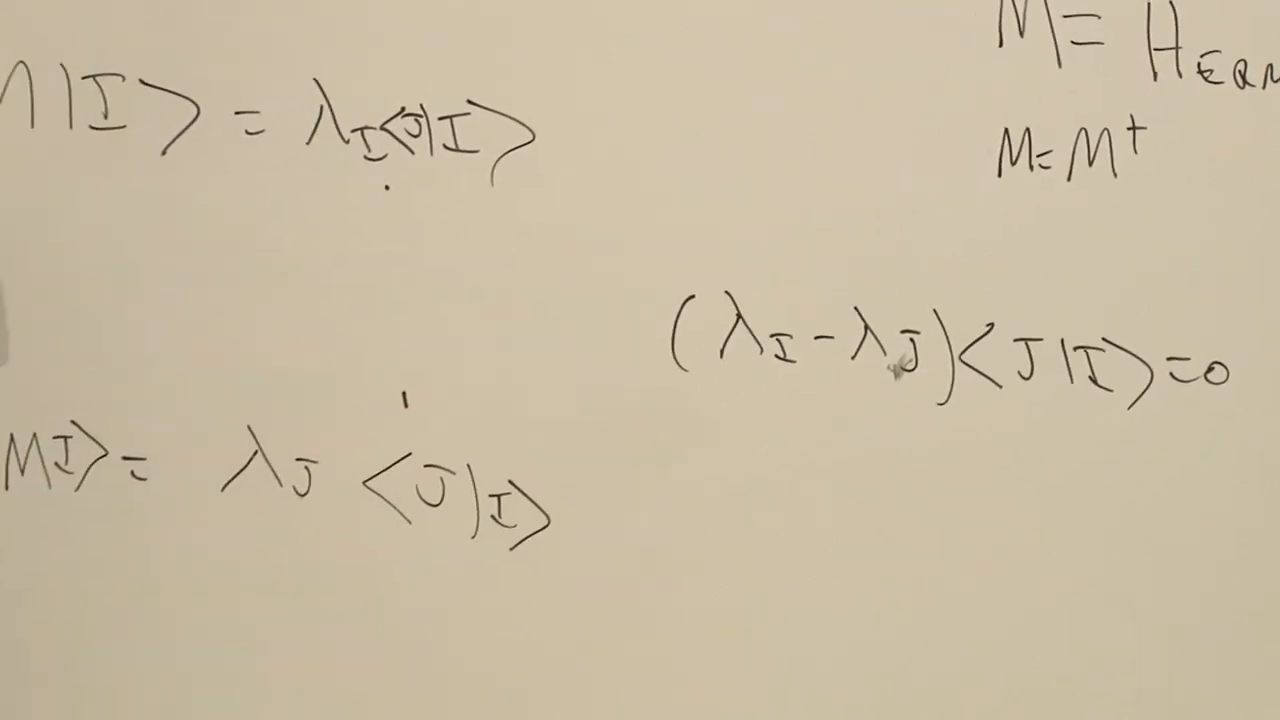
\includegraphics[width=0.82\textwidth]{lecture_03_figure_07.png}
\caption{正交性证明中的决定性一步：不相等的本征值迫使内积为零。}
\lectureframe{00:59:00}
\end{figure}

当两个本征值恰好相等时，式~\eqref{eq:hermitian-orthogonality}在该简并本征空间内不施加任何条件。可以在那里选择一个正交归一基。与其余本征方向一起，这些矢量构成谱定理所承诺的完全正交归一的本征基。

正交性也有物理解读。两个正交态可以通过适当的测量被无歧义地区分。具有不同本征值的本征态必定是可区分的，因为仪器对它们报告不同的实数。代数与操作意义已经指向同一对应关系。

\section{测量公设}

我们现在已有足够的形式体系来陈述基本的量子力学对应关系。它们初次遇到时可能听起来陌生。只有使用之后其含义才会变得具体，所以让我们干净地陈述它们，然后立刻回到自旋实验。

一次测量产生一个实数。人们可以把两个相容的实数读数打包成一个复数，但那个包仍然包含两次测量。一个探测器的基本输出是实的。因此厄米算符是自然的候选者：它们的本征值是实的，它们的本征矢量构成完全正交归一基。

\begin{enumerate}
\item 一个可测量量，或\emph{可观测量}，由厄米算符\(M\)表示。
\item 测量\(M\)的可能结果是它的本征值\(\lambda_i\)。
\item 其中\(M\)具有确定值\(\lambda_i\)的态是本征态\(\ket{i}\)，满足
\[
M\ket{i}=\lambda_i\ket{i}.
\]
\item 如果系统处于一般归一化态\(\ket{A}\)，那么得到\(\lambda_i\)的概率是
\begin{equation}
P(\lambda_i\mid A)
=\left|\braket{i}{A}\right|^2
=\braket{i}{A}\braket{A}{i}.
\label{eq:born-rule}
\end{equation}
\end{enumerate}

这个列表是方便的出发点，不一定是极小独立公理系统；用更经济的表述，有些陈述可以从其他陈述推导出来。将这些对应关系分开陈述，更容易看出它们的物理作用。

复数\(\braket{i}{A}\)是一个\emph{概率幅}，而不是概率。用它乘以自身的复共轭得到一个实的非负数。对于一个自旋分量，谱只有两个值，\(+1\)和\(-1\)；更一般的可观测量可以有许多本征值。

\begin{figure}[htbp]
\centering
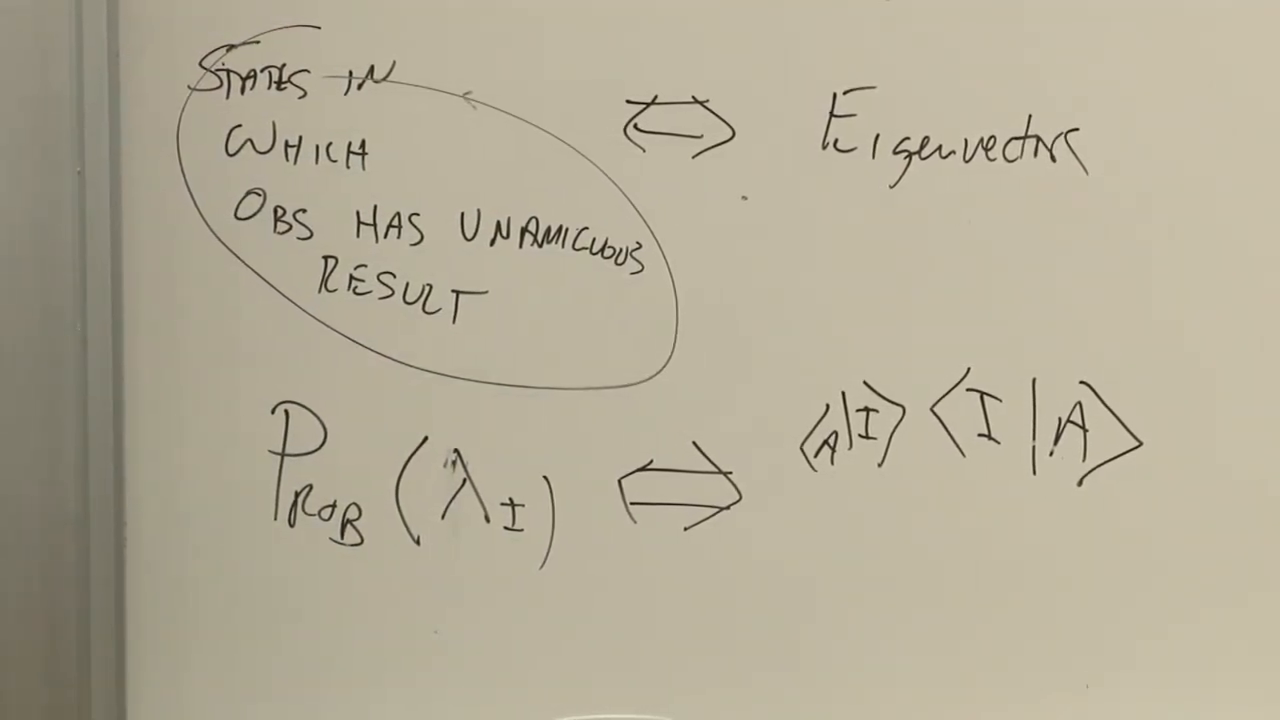
\includegraphics[width=0.82\textwidth]{lecture_03_figure_08.png}
\caption{黑板将确定结果态与本征向量联系起来，并将\(\lambda_i\)的概率与到\(\ket{i}\)上的投影的平方联系起来。}
\lectureframe{01:11:29}
\end{figure}

\begin{classroomqa}
\audiencequestion{在概率规则中，\(P\)旁边究竟写的是什么？}
\lecturerresponse{是\(\lambda_i\)：\(P(\lambda_i\mid A)\)表示当系统被制备在\(\ket{A}\)时，对\(M\)的测量返回特定本征值\(\lambda_i\)的概率。右边是到该本征向量上的投影的模平方。}
\end{classroomqa}

\subsection{归一化与完备性}

所有互斥结果的概率之和必须为一：
\begin{equation}
\sum_i\left|\braket{i}{A}\right|^2=1.
\label{eq:probability-normalization}
\end{equation}
代入完备本征基：
\begin{align}
\sum_i\left|\braket{i}{A}\right|^2
 &=\sum_i\braket{A}{i}\braket{i}{A}\\
 &=\bra{A}\left(\sum_i\ket{i}\bra{i}\right)\ket{A}\\
 &=\braket{A}{A}.
\end{align}
因此，允许的态矢量是归一化的，
\begin{equation}
\braket{A}{A}=1.
\label{eq:state-normalization}
\end{equation}
若\(\ket{A}=\sum_i\alpha_i\ket{i}\)，同一条件为
\begin{equation}
\sum_i\alpha_i^*\alpha_i=1.
\label{eq:component-normalization}
\end{equation}
这是对复分量的一个实约束。

\begin{classroomqa}
\audiencequestion{每个概率都必须为正吗？}
\lecturerresponse{是的。每个概率是一个数乘以它自己的复共轭，因此是非负的。归一化进而使所有这类数之和等于一。}
\end{classroomqa}

还有另一种冗余。将每个分量乘以同一相位，
\begin{equation}
\ket{A}\longmapsto e^{i\theta}\ket{A},
\label{eq:l3-global-phase}
\end{equation}
会使每个振幅乘以\(e^{i\theta}\)，而每个模平方保持不变。没有任何测量能探测到那个公共相位。分量之间的相对相位仍然是物理的；只有乘在整个态上的相位是冗余的。

因此，任意复矢量中的两个实参数并不指定物理态：其模由归一化固定，而其整体相位不可观测。这与单个自旋所遇到的参数计数相同，现在是从一般概率规则推导出来的。

\subsection{测量也进行制备}

还有一条公设，说起来容易，压缩成黑板上的一行短句却难。如果一次测量返回\(\lambda_i\)，那么紧接着系统处于相应的本征态\(\ket{i}\)。仪器既记录一个结果，又制备出一个态，在其中重复同一测量会得到那个确定结果。

\begin{classroomqa}
\audiencequestion{那个测量—制备的陈述能再说一遍吗？}
\lecturerresponse{在测量之前，若干本征值可能以式~\eqref{eq:born-rule}中的概率出现。一旦仪器实际报告\(\lambda_i\)，系统就被留在属于\(\lambda_i\)的本征态中。因此，对同一可观测量的第二次立即测量会返回同一个值。}
\end{classroomqa}

\begin{classroomqa}
\audiencequestion{这些原理已经告诉我们态如何随时间演化了吗？}
\lecturerresponse{还没有。我们已经规定了态是什么、可观测量如何表示，以及测量做什么。支配随时间变化的定律是额外的结构，将在后面引入。这类似于先定义经典相空间，再写出运动方程。}
\end{classroomqa}

\begin{classroomqa}
\audiencequestion{先前沿倾斜轴的平均自旋涉及\(\cos\theta\)。新的振幅平方规则是否应使它成为\(\cos^2\theta\)？}
\lecturerresponse{概率和平均值是不同的量。平均值把\(+1\)和\(-1\)两种结果的概率连同它们的符号结合起来。一旦构造出任意方向的自旋量，振幅平方就会重现先前的余弦平均值。那个计算是下一个应用，而不是通过改变旧公式来猜测的东西。}
\end{classroomqa}

\section{自旋作为第一个应用}

三个可测量的自旋分量由厄米算符表示
\[
\sigma_x,\qquad \sigma_y,\qquad \sigma_z.
\]
分析器实验已经给出了它们的可能取值和确定值态：
\[
\begin{array}{c|c|c}
\text{observable}&\text{eigenvalue }+1&\text{eigenvalue }-1\\ \hline
\sigma_z&\ket{u}&\ket{d}\\
\sigma_x&\ket{r}&\ket{l}\\
\sigma_y&\ket{\mathrm{in}}&\ket{\mathrm{out}}
\end{array}
\]
这些信息足以把算符重构为矩阵。

\subsection{本征基中的 z 分量}

选择上--下基。确定的\(z\)自旋意味着
\begin{equation}
\sigma_z\ket{u}=+\ket{u},
\qquad
\sigma_z\ket{d}=-\ket{d}.
\label{eq:sigma-z-eigenvectors}
\end{equation}
两个本征值不同，因此厄米性意味着\(\braket{u}{d}=0\)。

计算四个矩阵元：
\begin{align}
\bra{u}\sigma_z\ket{u}&=+1,&
\bra{u}\sigma_z\ket{d}&=-\braket{u}{d}=0,\\
\bra{d}\sigma_z\ket{u}&=\braket{d}{u}=0,&
\bra{d}\sigma_z\ket{d}&=-1.
\end{align}
因此
\begin{equation}
\boxed{
\sigma_z=
\begin{pmatrix}
1&0\\
0&-1
\end{pmatrix}_{\{u,d\}}.}
\label{eq:sigma-z}
\end{equation}
坐标列是
\[
\ket{u}\widehat{=}\begin{pmatrix}1\\0\end{pmatrix},
\qquad
\ket{d}\widehat{=}\begin{pmatrix}0\\1\end{pmatrix}.
\]
乘以式~\eqref{eq:sigma-z}使第一列保持不变，使第二列带一个负号，正好符合本征值方程的要求。

\begin{figure}[htbp]
\centering
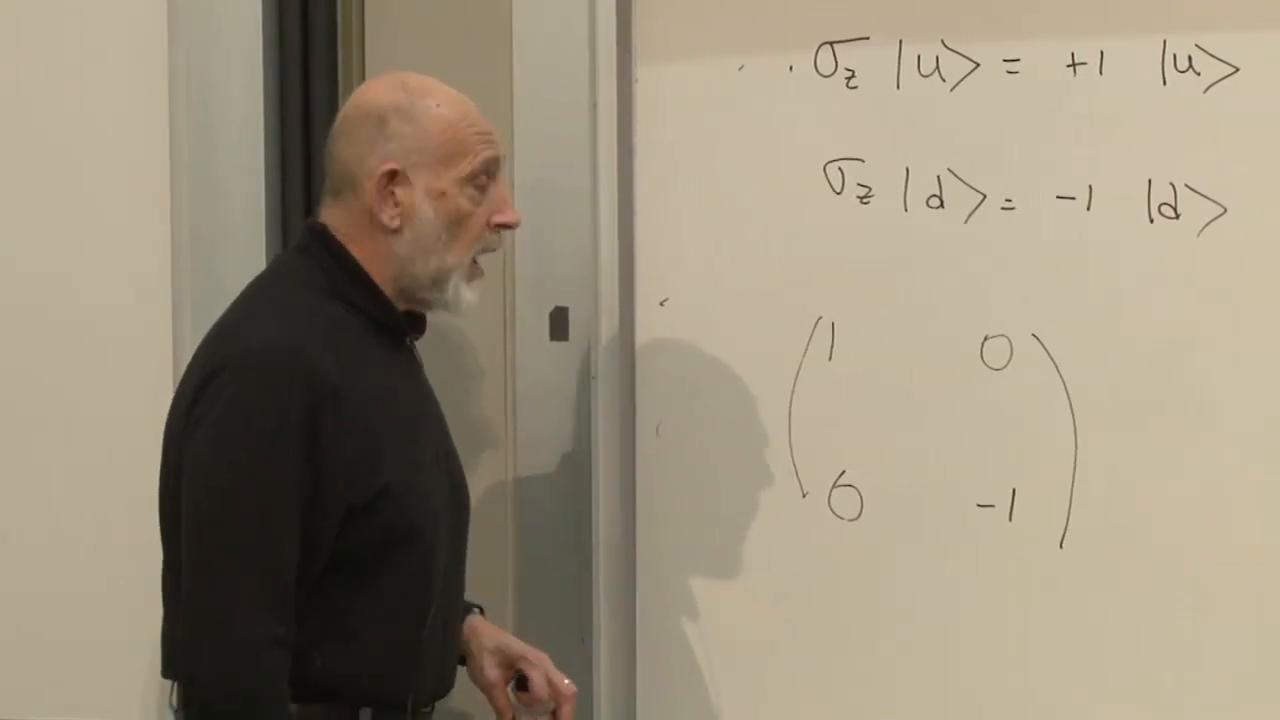
\includegraphics[width=0.82\textwidth]{lecture_03_figure_09.png}
\caption{在上--下基下，\(\sigma_z\)的本征方程及由此得到的对角矩阵。}
\lectureframe{01:26:56}
\end{figure}

\subsection{不改变基的x分量}

在右--左基下，\(\sigma_x\)也会具有相同的对角形式。那样做很容易，但得不到什么信息。保持上--下基，并使用
\begin{equation}
\sigma_x\ket{r}=+\ket{r},
\qquad
\sigma_x\ket{l}=-\ket{l}.
\label{eq:sigma-x-eigenvectors}
\end{equation}
两个基之间的关系为
\begin{align}
\ket{r}&=\frac{\ket{u}+\ket{d}}{\sqrt2},&
\ket{l}&=\frac{\ket{u}-\ket{d}}{\sqrt2},\\
\ket{u}&=\frac{\ket{r}+\ket{l}}{\sqrt2},&
\ket{d}&=\frac{\ket{r}-\ket{l}}{\sqrt2}.
\label{eq:x-z-basis-relations}
\end{align}

从对角元的上方元素开始：
\begin{align}
\bra{u}\sigma_x\ket{u}
 &=\frac12(\bra{r}+\bra{l})\sigma_x(\ket{r}+\ket{l})\\
 &=\frac12(\bra{r}+\bra{l})(\ket{r}-\ket{l})\\
 &=0.
\end{align}
右态和左态是正交归一的，因此两个对角项相消，交叉项为零。对\(\ket{d}\)做同样的计算得到
\[
\bra{d}\sigma_x\ket{d}=0.
\]
此时两个零并不意味着算符为零；它们告诉我们去看非对角元。

对于右上元素，
\begin{align}
\bra{u}\sigma_x\ket{d}
 &=\frac12(\bra{r}+\bra{l})\sigma_x(\ket{r}-\ket{l})\\
 &=\frac12(\bra{r}+\bra{l})(\ket{r}+\ket{l})\\
 &=1.
\end{align}
厄米性，或者直接重复该计算，给出
\[
\bra{d}\sigma_x\ket{u}=1.
\]
因此
\begin{equation}
\boxed{
\sigma_x=
\begin{pmatrix}
0&1\\
1&0
\end{pmatrix}_{\{u,d\}}.}
\label{eq:sigma-x}
\end{equation}
同一个抽象算符在它自己的本征基下是对角的，而在\(z\)基下是非对角的。这是基依赖性不带来物理歧义的一个具体实例。

\subsection{y分量与相对相位}

选择归一化的入--出约定
\begin{equation}
\ket{\mathrm{in}}=\frac{\ket{u}+i\ket{d}}{\sqrt2},
\qquad
\ket{\mathrm{out}}=\frac{\ket{u}-i\ket{d}}{\sqrt2},
\label{eq:l3-in-out-states}
\end{equation}
其中
\[
\sigma_y\ket{\mathrm{in}}=+\ket{\mathrm{in}},
\qquad
\sigma_y\ket{\mathrm{out}}=-\ket{\mathrm{out}}.
\]
交换标签或反转\(y\)轴改变的是符号约定，而不是底层的构造。利用式~\eqref{eq:l3-in-out-states}，以这些本征矢和本征值为本征矢与本征值的唯一厄米矩阵为
\begin{equation}
\boxed{
\sigma_y=
\begin{pmatrix}
0&-i\\
i&0
\end{pmatrix}_{\{u,d\}}.}
\label{eq:sigma-y}
\end{equation}
容易验证而不必重新推导：
\begin{align}
\begin{pmatrix}0&-i\\i&0\end{pmatrix}
\frac1{\sqrt2}\begin{pmatrix}1\\i\end{pmatrix}
&=\frac1{\sqrt2}\begin{pmatrix}1\\i\end{pmatrix},\\
\begin{pmatrix}0&-i\\i&0\end{pmatrix}
\frac1{\sqrt2}\begin{pmatrix}1\\-i\end{pmatrix}
&=-\frac1{\sqrt2}\begin{pmatrix}1\\-i\end{pmatrix}.
\end{align}
因子\(1/\sqrt2\)使本征矢归一化，但不影响它们的本征方向。

\begin{figure}[htbp]
\centering
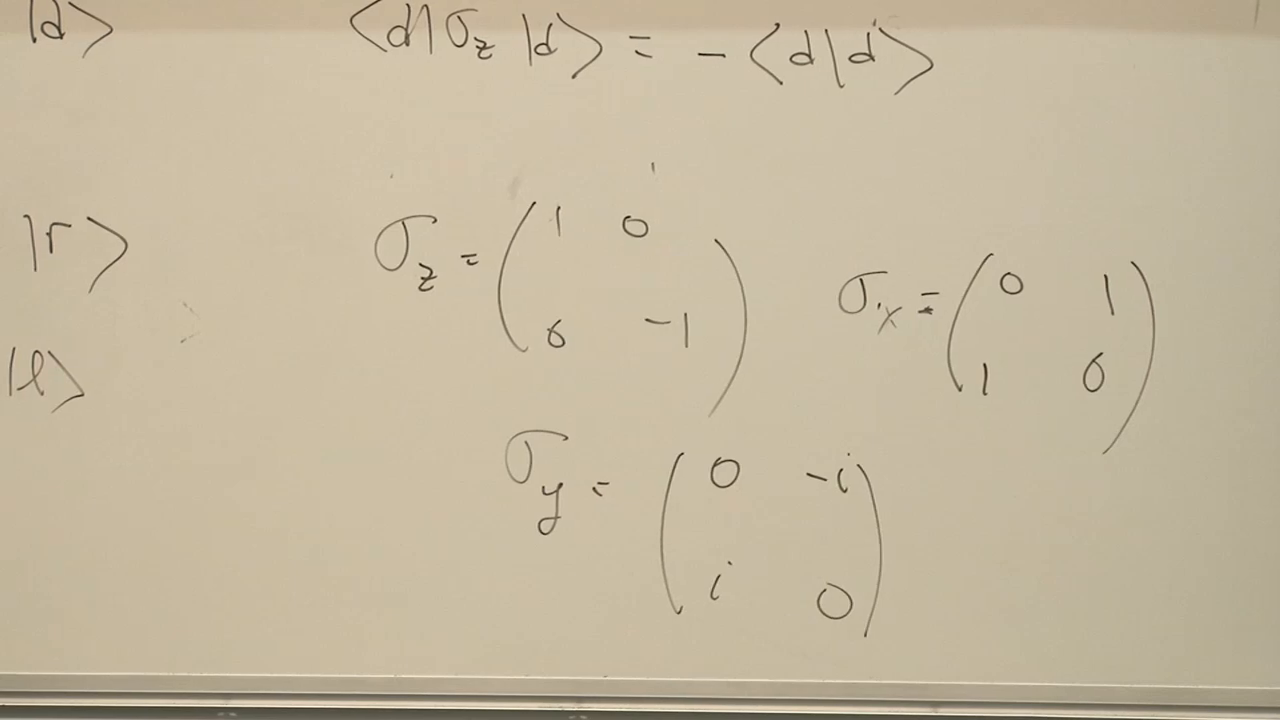
\includegraphics[width=0.82\textwidth]{lecture_03_figure_10.png}
\caption{在上--下基下完整的板书泡利矩阵集合。}
\lectureframe{01:38:11}
\end{figure}

\begin{classroomqa}
\audiencequestion{是否应改变入--出矢量中的一个符号以使它们正交？}
\lecturerresponse{不。缺失的一步是把右矢变成左矢时的复共轭：
\[
\bra{\mathrm{in}}=\frac{\bra{u}-i\bra{d}}{\sqrt2}.
\]
因此
\[
\begin{aligned}
\braket{\mathrm{in}}{\mathrm{out}}
&=\frac12(\bra{u}-i\bra{d})
  (\ket{u}-i\ket{d})\\
&=\frac12\bigl(1+(-i)(-i)\bigr)\\
&=0.
\end{aligned}
\]
忘记这一共轭正是左矢--右矢记号所要揭示的常见错误。}
\end{classroomqa}

我们已经得到
\begin{equation}
\begin{aligned}
\sigma_x&=\begin{pmatrix}0&1\\1&0\end{pmatrix},\\[0.4em]
\sigma_y&=\begin{pmatrix}0&-i\\i&0\end{pmatrix},\\[0.4em]
\sigma_z&=\begin{pmatrix}1&0\\0&-1\end{pmatrix}.
\end{aligned}
\label{eq:pauli-triple}
\end{equation}
它们都是厄米的，本征值为\(\pm1\)，并且恰好具有分析器实验所要求的确定自旋本征矢。

下一个问题现在提得很明确。给定一个沿任意方向制备的自旋，构造相应的态，并用振幅的平方计算\(\sigma_z=+1\)和\(\sigma_z=-1\)的概率。形式体系已经包含足够的信息；进行这一计算是自然的下一步。
